\documentclass{beamer}
\usetheme[progressbar=frametitle]{metropolis}           % Use metropolis theme
% \setbeamercolor{progress bar}{fg=green,bg=blue}


\usepackage[backend=biber,style=alphabetic,citestyle=authoryear]{biblatex}
\usepackage{graphicx}
\usepackage[T1]{fontenc}
\usepackage[utf8]{inputenc}
\usepackage[english]{babel}



% % Alter some LaTeX defaults for better treatment of figures:
% % See p.105 of "TeX Unbound" for suggested values.
% % See pp. 199-200 of Lamport's "LaTeX" book for details.
% %   General parameters, for ALL pages:
% \renewcommand{\topfraction}{0.9}	% max fraction of floats at top
% \renewcommand{\bottomfraction}{0.8}	% max fraction of floats at bottom
% %   Parameters for TEXT pages (not float pages):
% \setcounter{topnumber}{2}
% \setcounter{bottomnumber}{2}
% \setcounter{totalnumber}{4}     % 2 may work better
% \setcounter{dbltopnumber}{2}    % for 2-column pages
% \renewcommand{\dbltopfraction}{0.9}	% fit big float above 2-col. text
% \renewcommand{\textfraction}{0.07}	% allow minimal text w. figs
% %   Parameters for FLOAT pages (not text pages):
% \renewcommand{\floatpagefraction}{0.7}	% require fuller float pages
% % N.B.: floatpagefraction MUST be less than topfraction !!
% \renewcommand{\dblfloatpagefraction}{0.7}	% require fuller float pages
% % remember to use [htp] or [htpb] for placement

% \setbeamertemplate{headline}{%
%   \begin{beamercolorbox}[colsep=1.5pt]{upper separation line head}
%   \end{beamercolorbox}
%   \begin{beamercolorbox}{section in head/foot}
%     \vskip2pt\insertnavigation{\paperwidth}\vskip2pt
%   \end{beamercolorbox}%
%   \begin{beamercolorbox}[colsep=1.5pt]{lower separation line head}
%   \end{beamercolorbox}
% }
% \setbeamercolor{section in head/foot}{fg=normal text.bg, bg=structure.fg}



\title{Major steps and future challenges of numerical weather prediction}
\date{\today}
\author{Eirik Gallefoss}

% \titlegraphic{
\includegraphics[width=2cm]{../figures/uio-logo.jpg}\hspace*{4cm}~%
% }


\institute{Geologisk institutt - Universitetet i Oslo}



\expandafter\def\expandafter\insertshorttitle\expandafter{%
  \insertshorttitle\hfill%
  \insertframenumber\,/\,\inserttotalframenumber}


  \setbeamertemplate{section in toc}[sections numbered]

\addbibresource{references.bib}

\begin{document}

\begin{frame}
  \titlepage
\end{frame}


\begin{frame}
  \frametitle{Overview}
  % \tableofcontents
  % \tableofcontents[currentsection]
  \tableofcontents
\end{frame}


\section{Introduction}
  \begin{frame}{First Frame}
    Hello, world!
  \end{frame}

\section{Historical overview}

\begin{frame}{}
  \begin{itemize}
    \item Bjerknes 1904
    \item Richardson 1922
    \item Charney, Fjørtoft, von Neumann 1950
    \item Rossby 1954

    \item Charney/U.S. Weather Bureau 1955
    \item Shuman 1966
    \item 1990
    \item Today

  \end{itemize}
\end{frame}


\section{Past breakthroughs}

\begin{frame}{Model initialization}
  \begin{figure}[H]
    \centering
    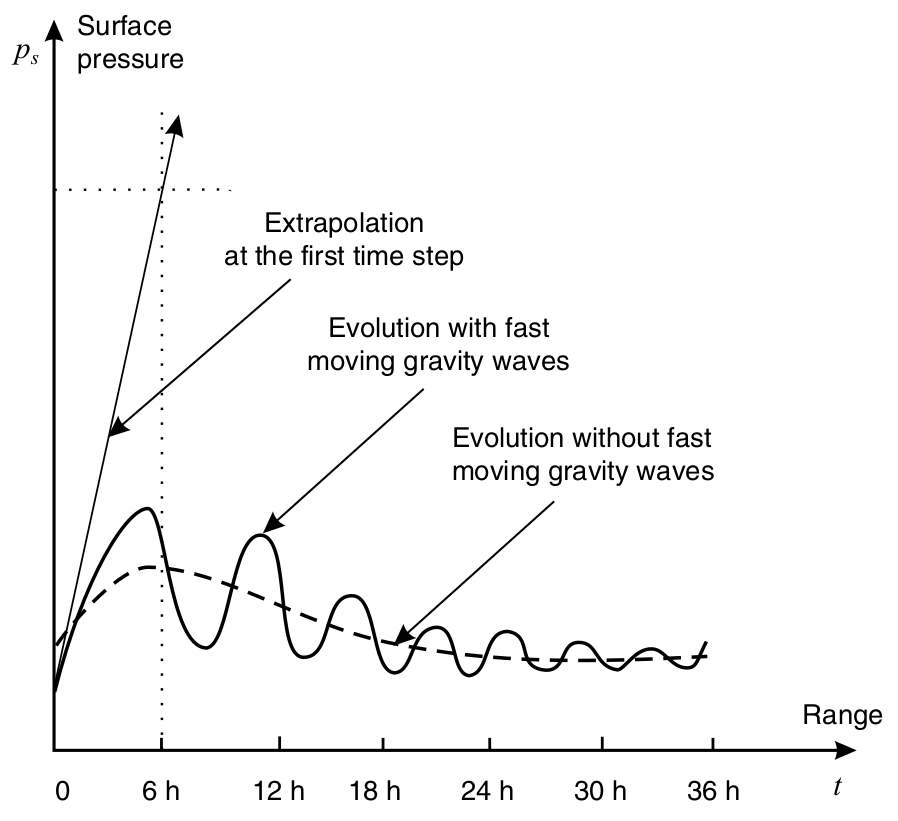
\includegraphics[width=0.6\textwidth]{../figures/nwp_pressure}

    \parencite{nwp}
  \end{figure}

\end{frame}


\begin{frame}{Physical processes}
  \begin{figure}[H]
    \centering
    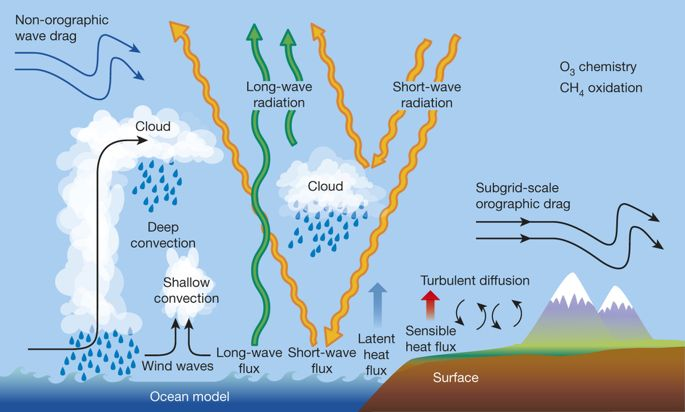
\includegraphics[width=0.8\textwidth]{../figures/bauer_physical.jpg}

    \parencite{bauer}
  \end{figure}
\end{frame}


\begin{frame}{Computational power}

  \begin{itemize}
    \item Model run time
    \item CFL-criteria
  \end{itemize}

  $$ T = \frac{N_v N_c N_t}{R}$$

  $$ \frac{U \Delta t}{\Delta x} < C $$

\end{frame}

\section{Future challenges}

\begin{frame}{Computational challenges}
  \begin{figure}[htp]
    \centering
    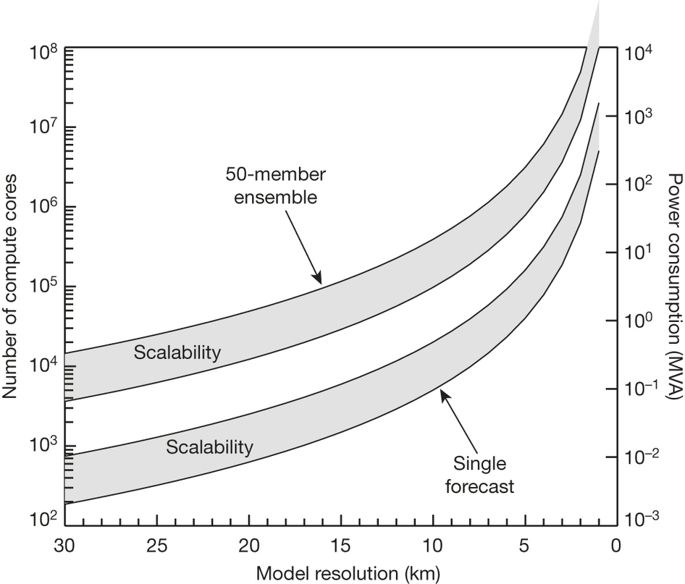
\includegraphics[width=0.6\textwidth]{../figures/bauer_cpu.jpg}

  \parencite{bauer}
  \end{figure}
\end{frame}

\begin{frame}{References}
  \printbibliography
\end{frame}

\end{document}
